% TEMPLATE for Usenix papers, specifically to meet requirements of
%  USENIX '05
% originally a template for producing IEEE-format articles using LaTeX.
%   written by Matthew Ward, CS Department, Worcester Polytechnic Institute.
% adapted by David Beazley for his excellent SWIG paper in Proceedings,
%   Tcl 96
% turned into a smartass generic template by De Clarke, with thanks to
%   both the above pioneers
% use at your own risk.  Complaints to /dev/null.
% make it two column with no page numbering, default is 10 point

% Munged by Fred Douglis <douglis@research.att.com> 10/97 to separate
% the .sty file from the LaTeX source template, so that people can
% more easily include the .sty file into an existing document.  Also
% changed to more closely follow the style guidelines as represented
% by the Word sample file. 

% Note that since 2010, USENIX does not require endnotes. If you want
% foot of page notes, don't include the endnotes package in the 
% usepackage command, below.

% This version uses the latex2e styles, not the very ancient 2.09 stuff.
\documentclass[letterpaper,twocolumn,10pt]{article}
\usepackage{graphicx}
\usepackage{usenix,epsfig}
\usepackage{url}


\begin{document}

%don't want date printed
\date{}

%make title bold and 14 pt font (Latex default is non-bold, 16 pt)
\title{\Large \bf Automated Analysis of Election Audit Logs}

%for single author (just remove % characters)
\author{
% {\rm Your N.\ Here}\\
% Your Institution
% \and
% {\rm Second Name}\\
% Second Institution
% copy the following lines to add more authors
% \and
% {\rm Name}\\
%Name Institution
} % end author

\maketitle

% Use the following at camera-ready time to suppress page numbers.
% Comment it out when you first submit the paper for review.
%\thispagestyle{empty}


\subsection*{Abstract}
The voting audit logs produced by electronic voting systems contain data
that could be useful for uncovering procedural errors and election anomalies, but they
are currently unwieldy and difficult for election officials to use in
post-election audits. In this work, we develop new methods to analyze these
audit logs for the detection of both procedural errors and system
deficiencies. Our methods can be used to detect votes that were not included in
the final tally, machines that may have experienced hardware problems during the
election, and polling locations that closed late. We tested our analyses on
data from the South Carolina 2010 elections and were able to uncover, solely
through the analysis of audit logs, a variety of problems, including vote
miscounts. We created a public web application that applies these methods to
uploaded audit logs and generates useful feedback on any detected issues.


\section{Introduction}
A Direct Recording Electronic (DRE) voting machine is one in which the voter
interacts directly with the terminal, typically through a touch screen. DREs
provide a friendly interface to assist the voter with the ballot marking
process. DRE machines can issue electronic ballots on demand; running out of
paper ballots is no longer an issue. Additionally, audio DREs can assist
visually impaired voters.

Federal standards require that electronic voting machines generate detailed
audit logs for use during post-election audits. Unfortunately, while the logs
contain large amounts of data, it is not immediately obvious what sort of useful
information can be learned from the data. Furthermore, even simple
tallies are cumbersome, time consuming, and prone to human error if done
manually. For these reasons, election officials do not regularly perform
countywide post-election analysis of the log data.

In this work, we aim to make DRE audit log analysis more useful and accessible
to election officials and other interested parties. We develop new methods to
analyze audit logs for the detection of both procedural errors and system
deficiencies. We created AuditTool\footnote{The name of the tool has been
  blinded for anonymous submission.}, a public web application that provides our 
analyses as a free service for use by election officials or interested third
parties.  

A strength of our tool is that even in the face of missing data, we still are 
able to pull out useful imformation. Our research contributes to the election 
audit process in the following ways.

\begin{itemize}
\item We introduce methods for identifying, solely from publicly available audit
  logs, potential errors in the software, hardware, and system configuration of
  DREs .
\item We introduce methods for identifying instances of human error by poll
  workers. Furthermore, we show how to differentiate between random
  errors and patterns of error that suggest shortcomings in the training
  election workers receive.
\item We introduce a new method for conducting a statistical analysis of voter
  flow. This allows for improved resource allocation in future elections.
\item We conduct a case study using our methods and identify instances of poor
  worker training, long voting lines, and missing votes during the 2010 South
  Carolina election.
\item Using our experience with the case study, we suggest new content that, if
  included in election log files, would allow for additional useful analysis.
\end{itemize}

We implement these methods for the ES\&S 
iVotronic DRE; the 2010 South Carolina data was already publicly available 
through a previous Freedom of Information Act request and the iVotronic was 
used in that election. The iVotronic system is a standalone, portable, 
touchscreen system that records vote totals, ballot images and an event log 
on internal flash memory. The iVotronic voting machine is one of the most 
widely deployed DREs in the U.S. In 2010, 422 jurisdictions tallying more 
than 22 million registered voters used this system~\cite{VerVot2010}. In 
addition, the types of analyses we identify and our algorithms for analysis 
are applicable to other DRE voting systems that produce the necessary audit 
logs. We show how the audit log data can be used to detect votes that may 
have been left out of the official results, incorrect procedures being 
followed at the precincts, precincts that had to stay open late, and even 
errors in the collection of the audit data itself. These reports can help 
election officials and fair election advocacy groups better understand the 
events that took place during and after an election. 

In this work we assume that DRE audit logs are complete, accurate, trustworthy,
and free of accidental or malicious tampering. Detecting and preventing audit
log tampering is outside the scope of this work. 


\section{Background}
\subsection{Introduction to the iVotronic DRE}
A brief description of the iVotronic's functionality and its main system
components follows.  

\begin{description}
\item{Voting terminal} The voting terminal is a stand-alone touchscreen voting
  unit. It is equipped with an internal battery and a removable compact flash
  card Personalized Electronic Ballot (PEB). The PEB is a proprietary cartridge
  required to operate the iVotronic terminal. Typically, counties deploy two
  types of PEBs to the precinct: a) a master PEB and b) an activator PEB. They
  are interchangeable, but poll workers are trained to keep them separate and
  use them for different purposes.
\begin{itemize}
\item{Master PEB} Poll workers use the master PEB to open and close all
  terminals on election day. When a terminal is closed, it uploads its vote
  totals onto the PEB inserted into it. The PEB accumulates the precinct totals
  so that they can later be uploaded and included in the official tally.
\item{Activator PEBs} Activator PEBs are used bypoll workers to activate ballots
  for voters. Each voter’s session with the voting terminal starts with a poll
  worker inserting an Activator PEB into the terminal. 
\end{itemize}
\item{Removable Compact Flash (CF) card} The CF cards are programmed at Election
  Central and installed in the back of the voting terminal prior to deployment
  at the polling location. They store the event log and ballot images when the
  terminal is closed for voting. Once the polls close, the CF cards are removed
  from the back of the terminal and delivered to election headquarters on
  election night.
\end{description}

\subsection{iVotronic Audit Data}
The ES\&S voting solution produces many log files, but in our analysis we focus
on three: the event log (EL152.lst), the ballot image file (EL155.lst), and the
system log (EL68a.lst). 

The event log (EL152.lst) comes from the removable CF card and contains audit
log entries from each iVotronic terminal used in the election. The log records,
in chronological order, all events that occurred on that machine during the
election. Each event log entry includes the iVotronic's terminal serial number,
the PEB's serial number, the date and time, the event that occurred and a
description of the event.

The ballot image file (EL155.lst) is also from the removable CF card and
contains all ballot images saved by the iVotronic terminals during the voting
process. The ballot images are segregated by precinct and terminal where the
votes were cast. 

The system log listing file (EL68a.lst) chronologically tracks activity in the
election reporting database at the election headquarters. It contains the totals
accumulated in the various precincts during election night reporting, as well as
any warnings or errors reported by the software during the tabulation
process. The system log also tracks the uploading of PEBs and CF cards to the
election-reporting database.

\section{Analysis}
Our system is structured as a set of analyses, each one designed to shed light
on one particular aspect of election and post-election activities. In this
section we present a description of our analyses. 

\subsection{Analyses of Interest}
We focus on analyses that we expect to be most useful to election officials or
interested third parties. First, since vote-counting is fundamental to
elections, we use the audit logs to detect if cast votes are being under- or
over-counted.

Second, we use audit logs to identify which polling locations had long lines or
had to stay open late to accommodate voters already in line. Long lines in the
voting place can deter voters from casting their ballot. Knowing when and where
to expect lines might help election officials better allocate resources at the
next election. 

Third, we identify a number of seemingly small election-day issues that could
negatively affect the accuracy and fairness of an election, including:
malfunctioning displays that go unnoticed, which might cause a voter to cast a
vote other than as intended; malfunctioning machines, which could result in
fewer working machines and longer lines at the polling place; and failure to
follow procedures on the part of poll workers, which can lead to loss of votes
when a machine is not correctly closed out.

\subsection{Algorithms}
We briefly describe here the algorithms used in each of our analyses. For the
majority of these we only consider data from election day between the hours of
7 A.M. and 7 P.M., which are the times that polls open and close in South
Carolina. In our preliminary analysis, we found examples of log entries with
seemingly incorrect timestamps. We identified two types of timestamp errors:
errors resulting from incorrectly set clocks and errors resulting from apparent
bugs in the timestamp mechanism itself. Given only a timestamp in the logs, it
is impossible to know whether it is correct; however, we developed a number of
heuristics to find those terminals that likely do have an incorrect clock. We
may miss some terminals with an incorrect clock, but we try to minimize the
number of false reports we give. We provide the user with a report detailing the
results of this timestamp analysis.  

AuditTool detects whether any votes were left out of the tally. We assume the
tabulation software is correct and instead use the audit logs to check that all
cast votes are entered into the tabulation software. Recall that each voting
terminal’s vote totals are loaded onto a PEB when polls are closed and then all
these PEBs’ data are loaded in to the election reporting database. There are two
points in this process where votes could be omitted: a terminal may be forgotten
and never closed, so that no PEB contains its vote totals; or a PEB used to
close a terminal might be forgotten and not uploaded to the database. We show
how to use the audit logs to detect both of these problems.  

When searching the audit logs for instances of PEBs that were not uploaded, we
compared the contents of the event log and ballot image files to that of the
systems log listing file. We first identify, by parsing the event log, the set
of PEBs used to close out voting terminals and then verify each one appears as
uploaded in the system log file. When a PEB is missing from the system log file,
we report the case because it signifies that the PEB was not uploaded and the
votes may not be in the certified totals.  

Looking for terminals that were never closed is a challenging problem:
essentially we need to identify events that are missing from the logs. We do
this by finding terminals that were opened, but never closed.  

AuditTool also reports on polling locations that stayed open late and that had
long lines throughout the day. To identify locations that stayed open past 7
P.M., AuditTool first compiles a list of every terminal in the event log file
for which the last vote was cast after 7 P.M. Then, using information from the
ballot image file, the algorithm groups terminals by polling location and
computes the mean time of the last cast vote for each group. We take the mean in
order to account for any chance error in the timestamps. Finally, we report which
polling locations stayed open late and also provide, for every county, a chart
detailing the number of polling locations that stayed open late and by how
long. 
	 		
Identifying locations that had lines throughout the day is trickier. We start by
positing that when there is a line of voters waiting, there will be very little
idle time for each machine between voters. We would like to identify windows of
time where this was the case for a particular polling location. (Note that this
does not allow us to differentiate between voters standing in line and voters
arriving in a steady stream that keeps the machines at maximum capacity. It is a
shortcoming of our approach, but seems difficult to avoid given only the log
data.) The analysis is complicated however, by the fact that the logs do not
record an event when a new ballot is activated for a voter, only when a ballot
is cast. Given the timestamps $t_1$ and $t_2$ of two cast vote events for voter
$v_1$ and voter $v_2$, it could be the case that $v_2$ walked up to the terminal
as soon as $v_1$ cast her vote and then spent $t_2-t_1$ minutes marking her
ballot before casting her vote. Or, it could be that the terminal was idle for
most of $t_2-t_1$ and at the last moment, voter $v_2$ approached the terminal,
quickly marked her ballot and then cast her vote. If we knew how long the
average voter took to mark her ballot we could use that to estimate the length
of the idle time between two consecutive cast vote events. We do not know that
information directly, but we can infer it from the logs we have. We know which
locations were open after 7 P.M. and we also know that a polling location should
only stay open late if there are people waiting in line at the official poll
closing time. We assume this protocol is followed, and we further assume that
the line moves efficiently, and therefore the terminals in a given location
experience no idle time between voters after 7 P.M. Finally, we assume the time
it takes to mark a ballot is a random variable and these late voters are a
random sample of the entire voting population for that precinct. Therefore the
average time it 
takes them to vote represents the time it takes the average voter in the
precinct to vote. We 
then look for other times throughout the day where the time between votes is
similar to or less than the time between votes after 7 P.M. Starting at 7 A.M.,
for each location, we look at each one hour window that starts on the hour and
compile the set $S_1$ of time-between-consecutive-votes for every machine in
that location during the window. Next we compare this set to $S_2$, the
time-between-consecutive-votes for every machine in that location after 7
P.M. Note that we only perform this analysis on locations that were open after 7
P.M. If the mean of $S_1$ is less than the mean of $S_2$, this suggests times in
$S_1$ were shorter than in $S_2$ and there possibly were long lines in that
window. We then perform the Mann Whitney U statistical test to determine whether
the observed difference in mean is due to chance error. For windows where the
two-tailed p-value is less than 0.05, there is evidence that the difference in
mean is real and there possibly were long lines during the window when $S_1$ was
collected.  

This test does make a fair number of assumptions, and we offer no proof that
they are valid. However, we feel they are not entirely unreasonable, and more
important, our goal here is not to prove there were lines, but merely to alert
election officials about the possibility of lines occurring at certain times
throughout the day. Election officials can use this information to help them
allocate resources for future elections.  

We also report on machines that had an uncalibrated display at the time when a
vote was cast; there is the possibility that those votes may not have been cast
as intended. When detecting votes cast on uncalibrated machines, we looked for
three specific events in the event log: a machine uncalibrated event, a vote
cast event, and a machine recalibrated event. We used a simple finite state
machine with states = {uncalibrated machine with no votes cast, uncalibrated
  machine with at least one vote cast, calibrated machine} and tracked the
current state of each terminal as we iterated through the event log. We then
report any machine that had ever been in the state ``uncalibrated machine with
at least one vote cast.'' 

The procedural errors we are concerned with are: not printing zero tapes,
casting votes with master PEBs, and opening and closing a machine with
different PEBs. For each polling location, we check that every machine in the
location recorded printing zero tapes, that each machine was opened and closed
with the same PEB, and that no PEB used to open or close a machine was also used
to cast a vote.  

Last, we consider how to detect missing data: audit data that was not recorded,
but should have been. In some cases, this may be impossible; if there is no
trace of a terminal in any of the logs, we have no way of knowing that its data
is missing given only the logs. We focused on the audit data for cast votes and
find votes for which either the cast vote event was missing or the ballot image
was missing. We can not detect a cast vote which is missing both the cast vote
event and the ballot image. For each voting terminal, we compare the number of
cast vote events in the event log with the number of ballot images in the system
log. We report those terminals where the two values are not equal as the logs
must be missing data from those machines.  

\section{Implementation}
We built a web application called AuditTool to give election officials and
advocacy groups easy access to our toolset. AuditTool requires the user to
upload an event log and a ballot images file; we strongly suggest they also
submit the system log to take advantage of the full range of analyses our tool
provides. AuditTool uses only publically available log data and does not store
any information from the logs, so does not endanger voter privacy.  

AuditTool produces reports that warn election officials about possible miscounts
or procedural errors. Each report provides details about the errors found and
explains the possible consequences of the error and suggests, where applicable,
steps the election officials might take to address the error.

\section{Results}
This section discusses our findings after running our tool on the audit logs
from the South Carolina 2010 General Election. We tested our analysis using log
files downloaded from the website titled “South Carolina Voting
Information.”\footnote{\url{www.scvotinginfo.com}} 

\subsection{Missing Votes}
Our analysis shows that a total of 15 PEBs containing 2082 votes were not
uploaded from the 14 counties that we audited in South
Carolina. Figure~\ref{fig:pebs-not-uploaded} summarizes the PEBs not uploaded
during the General 2010 elections.  

\begin{figure}[htbp]
\begin{center}
    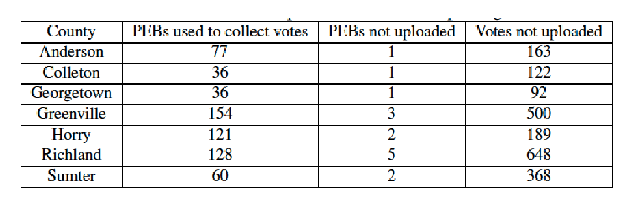
\includegraphics[width=0.5\textwidth,height=0.1\textheight]{PEBsNotUploaded1.eps}
\end{center}
\caption{PEBs not uploaded and their corresponding votes.}
\label{fig:pebs-not-uploaded}
\end{figure}

AuditTool also identified a few instances of machines not being closed. A
machine must be closed in order to collect the votes and audit data from that
machine. There was a single machine that wasn’t closed in each of the following
counties: Greenville County, Horry County, and Sumter County. If this was a
close election, information such as this could be cause for an extensive audit
or recount of the votes.  

Figure~\ref{fig:greenville-logs} shows some of AuditTool’s output on Greenville
County’s log files. 

\begin{figure}[htbp]
\begin{center}
    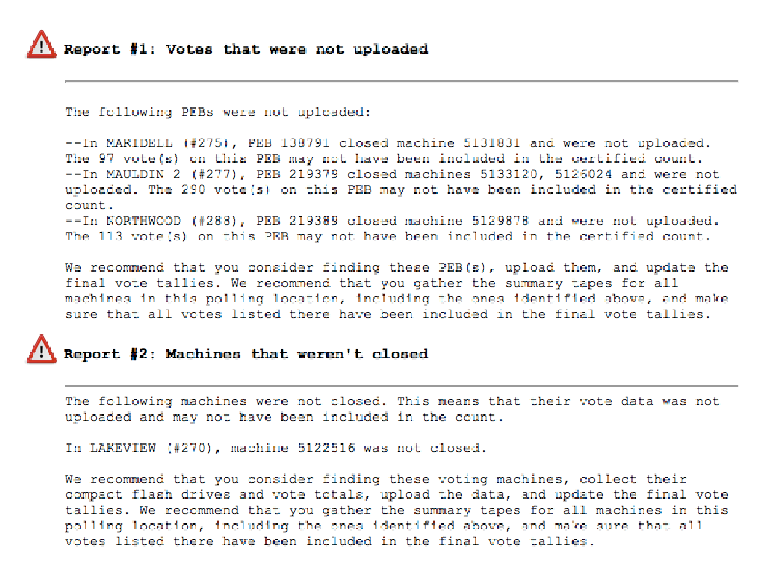
\includegraphics[width=0.5\textwidth,height=0.3\textheight]{VotesNotUploaded.eps}
\end{center}
\caption{Feedback for officials when detecting votes not having been uploaded.}
\label{fig:greenville-logs}
\end{figure}

\subsection{Calibration Errors}
 We found seven counties where at least one machine was possibly not calibrated
when votes were cast on that machine. An uncalibrated display could potentially
cause votes to not be cast as intended. Our report suggests an election official
or technician inspect these machines for possible calibration issues; see
Figure~\ref{fig:calibration-issues}.


\begin{figure}[htbp]
\begin{center}
    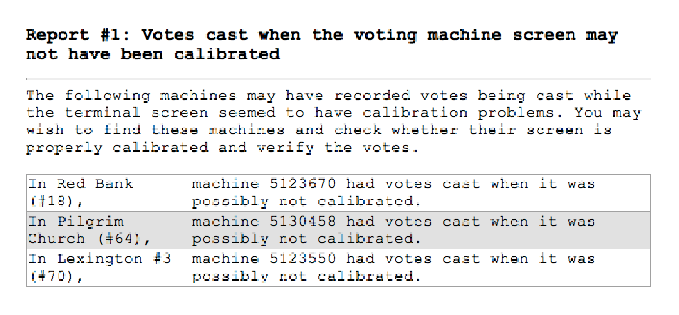
\includegraphics[width=0.5\textwidth,height=0.2\textheight]{NotCalibrated.eps}
\end{center}
\caption{Feedback for election officials when calibration issues are detected.}
\label{fig:calibration-issues}
\end{figure}

\subsection{Audit Data}
 In several counties, the audit logs appeared to be incomplete. Our analysis
 detected six counties that did not have the same set of machines in both the
 event log and ballot images file. Florence County had the most inconsistencies
 with 65 machines that had votes cast on them according to the event log, but no
 ballot images. We also saw cases where there were ballot images for votes cast
 on machines that did not record any events on the event log. In addition to an
 unusually large amount of missing data, the analysis of Florence County showed
 machines that did not have the same number of votes cast as ballot images. See
 Figure~\ref{fig:incomplete-audit-data} for example output from AuditTool. 

\begin{figure}[htbp]
\begin{center}
    
\includegraphics[width=0.5\textwidth,height=0.2\textheight]{IncompleteAuditData.eps}
\end{center}
\caption{Feedback when incomplete audit data is detected.}
\label{fig:incomplete-audit-data}
\end{figure}


\subsection{Procedural Errors}
Our findings reveal the need for improvements in poll worker training. When
opening and closing a machine, the same master PEB should be used, but in 11
counties there were machines opened and closed with different PEBs. Our results
showed a correlation between this error and certain precincts where poll workers
made those mistakes repeatedly. This indicates that perhaps the poll workers do
not know the procedures, whereas a random distribution of these errors across
polling locations probably means a mistake was made. Colleton County had five
instances of this procedural error, but four of those instances took place at
one polling location. Figure~\ref{fig:diff-pebs-open-close} shows this report
from Colleton County.  

A poll worker assigns each voter a PEB to use when it is that voter's turn. When 
voters cast votes, they should do so with a non-master PEB; we saw two counties 
that had an unusually high number of violations of this procedure. Horry County 
and Richland County had 22 and 32 instances of this violation, respectively. The
 feedback of this analysis for Richland County is shown in 
Figure~\ref{fig:master-peb-activated}. 

\begin{figure}[htbp]
\begin{center}
    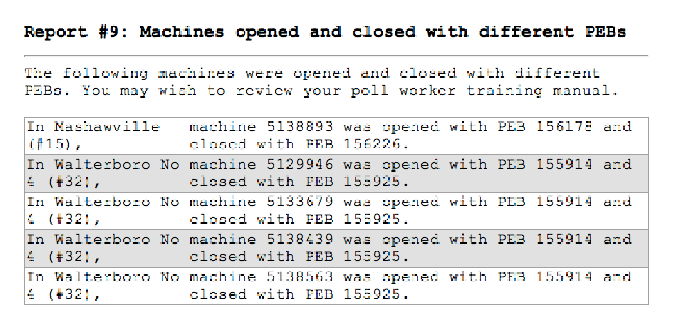
\includegraphics[width=0.5\textwidth,height=0.2\textheight]{OpenClosePEBs.eps}
\end{center}
\caption{AuditTool reports machines that were opened and closed with different PEBs.}
\label{fig:diff-pebs-open-close}
\end{figure}

\begin{figure}[htbp]
\begin{center}
    
\includegraphics[width=0.5\textwidth,height=0.4\textheight]{BallotsActivatedWithMasterPEB.eps}
\end{center}
\caption{AuditTool reports ballots activated with a master PEB.}
\label{fig:master-peb-activated}
\end{figure}

\subsection{Date/Time Errors}
 AuditTool found 1465 out of 4994 machines across 12 counties whose date was
 changed during election day voting. Figure~\ref{fig:one-hour-reset} shows an
 example of a 1-hour time change for Georgetown County. This county had 125 out
 of 140 machines adjusted nearly exactly one hour back in time. This suggests
 the wrong Daylight Savings Time algorithm was in use, as mentioned in previous
 audits~\cite{Buell2011}.

\begin{figure}[htbp]
\begin{center}
    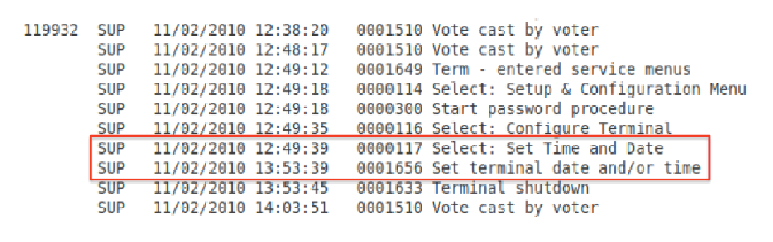
\includegraphics[width=0.5\textwidth,height=0.1\textheight]{ResetClock.eps}
\end{center}
\caption{Resetting an iVotronic clock by one hour in Georgetown County.}
\label{fig:one-hour-reset}
\end{figure}

Anomalous time changes were detected in 18 machines. An anomaly is any
occurrence of an unexplained date change while a machine is open for
voting. Figure~\ref{fig:date-anomaly} is an example that occurred in Richland
County. The machine was manually corrected about 30 minutes later.  

\begin{figure}[htbp]
\begin{center}
    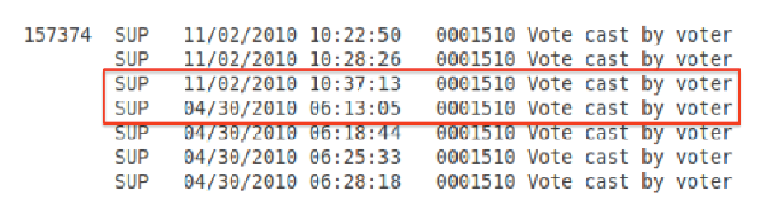
\includegraphics[width=0.5\textwidth,height=0.1\textheight]{DateAnomaly.eps}
\end{center}
\caption{This date anomaly occurred in Richland County during election day.}
\label{fig:date-anomaly}
\end{figure}

\subsection{Long Lines}
We found 671 out of a total of 942 South Carolina precincts stayed open
late. Berkeley County had the highest incidence of delayed closing times with
$93\%$ of polling locations closing after 7
P.M\@. Figure~\ref{fig:precincts-closed-late} depicts the precincts 
that closed late in Berkeley County. In the future, resources could be allocated
to those polling locations that stayed open the latest to help move their lines
more quickly. To detect possible lines before 7 P.M., we looked at only the
precincts that were open late. Figure~\ref{fig:long-lines} show the time periods
when the Berkeley County precincts experienced long lines before 7
P.M. Figure~\ref{fig:mann-whitney-u} shows the details of the results of the
Mann Whitney U statistical test for long lines.

\begin{figure}[htbp]
\begin{center}
    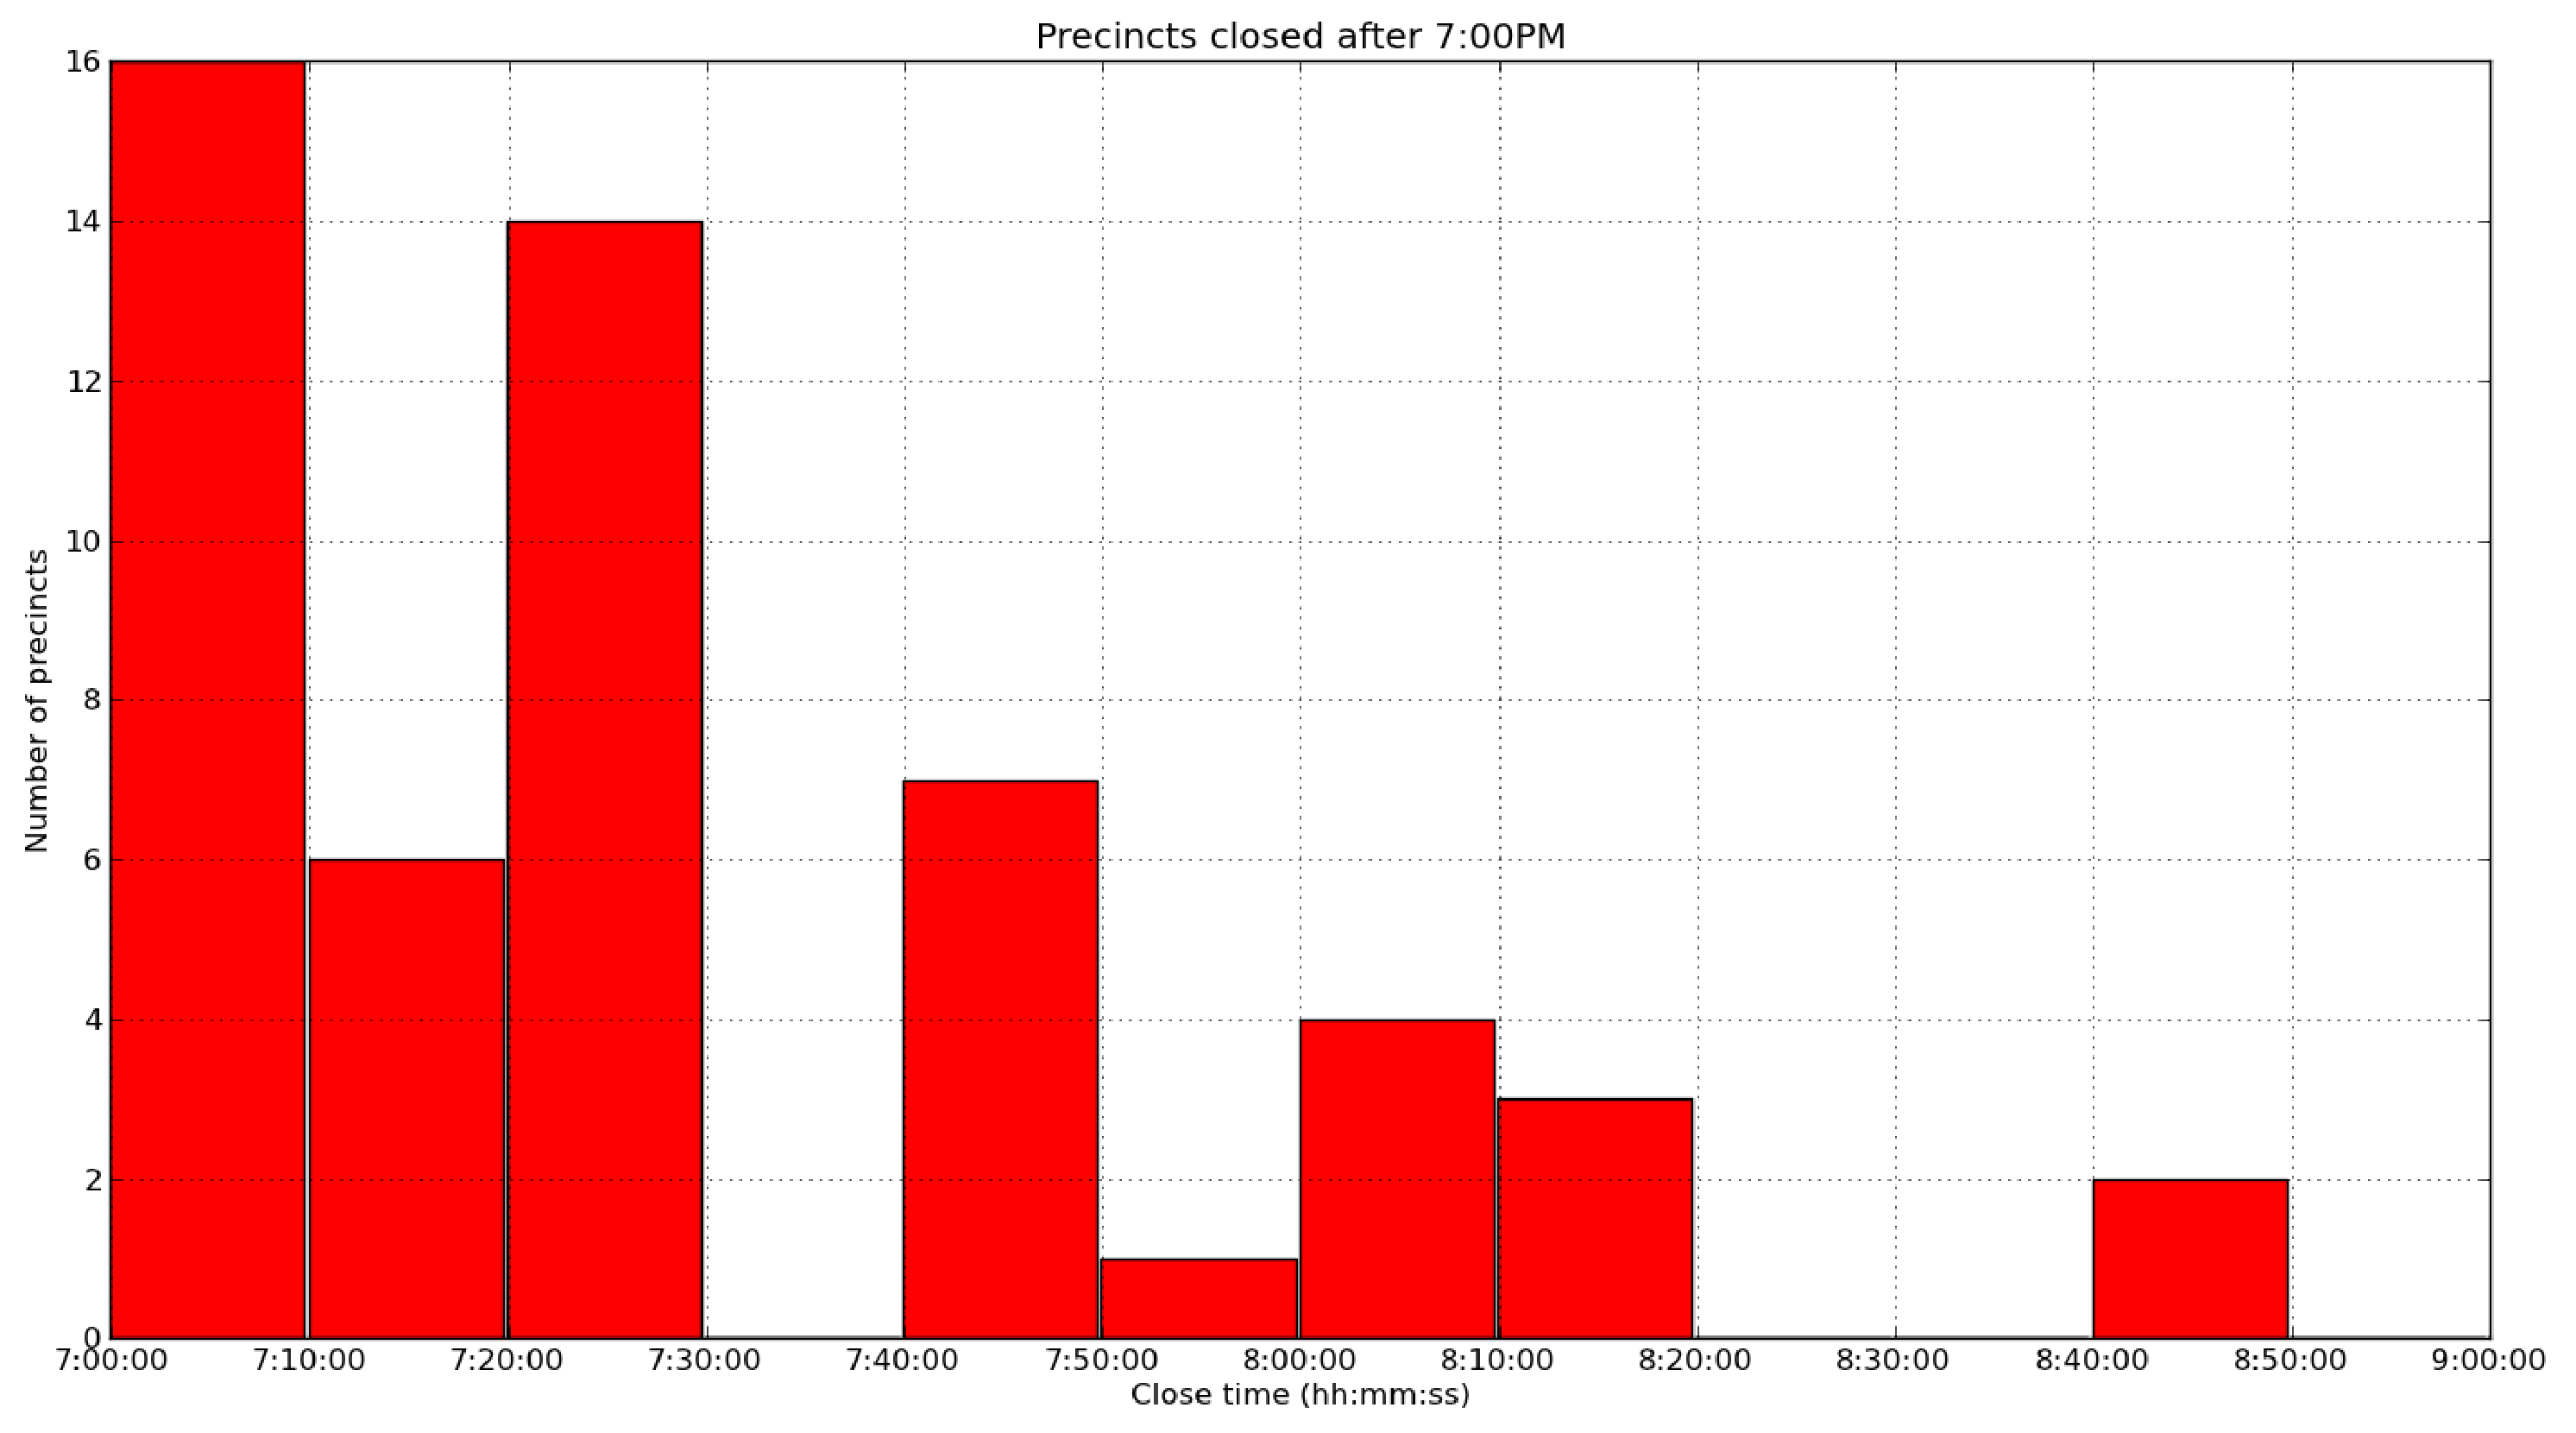
\includegraphics[width=0.5\textwidth,height=0.3\textheight]{berkeleyopenlate.eps}
\end{center}
\caption{Precincts that closed late in Berkeley County.}
\label{fig:precincts-closed-late}
\end{figure}

\begin{figure}[htbp]
\begin{center}
    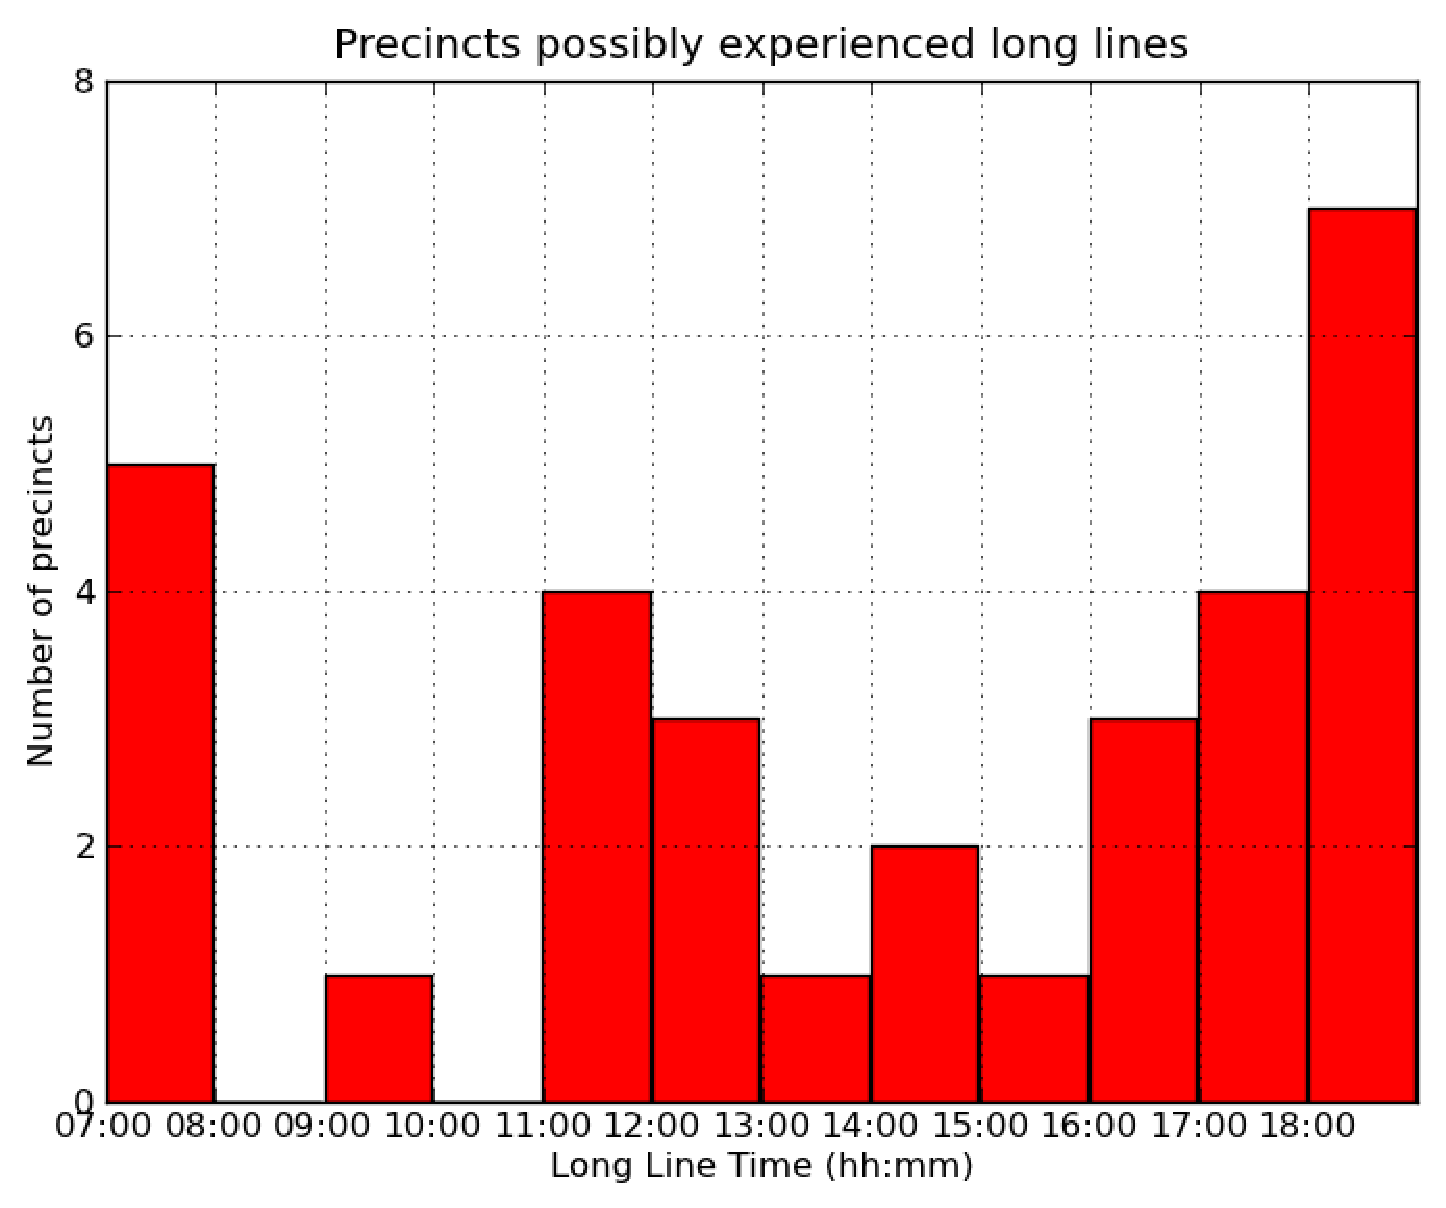
\includegraphics[width=0.5\textwidth,height=0.3\textheight]{berkeleyLongLine.eps}
\end{center}
\caption{Long lines in Berkeley County.}
\label{fig:long-lines}
\end{figure}

\begin{figure}[htbp]
\begin{center}
    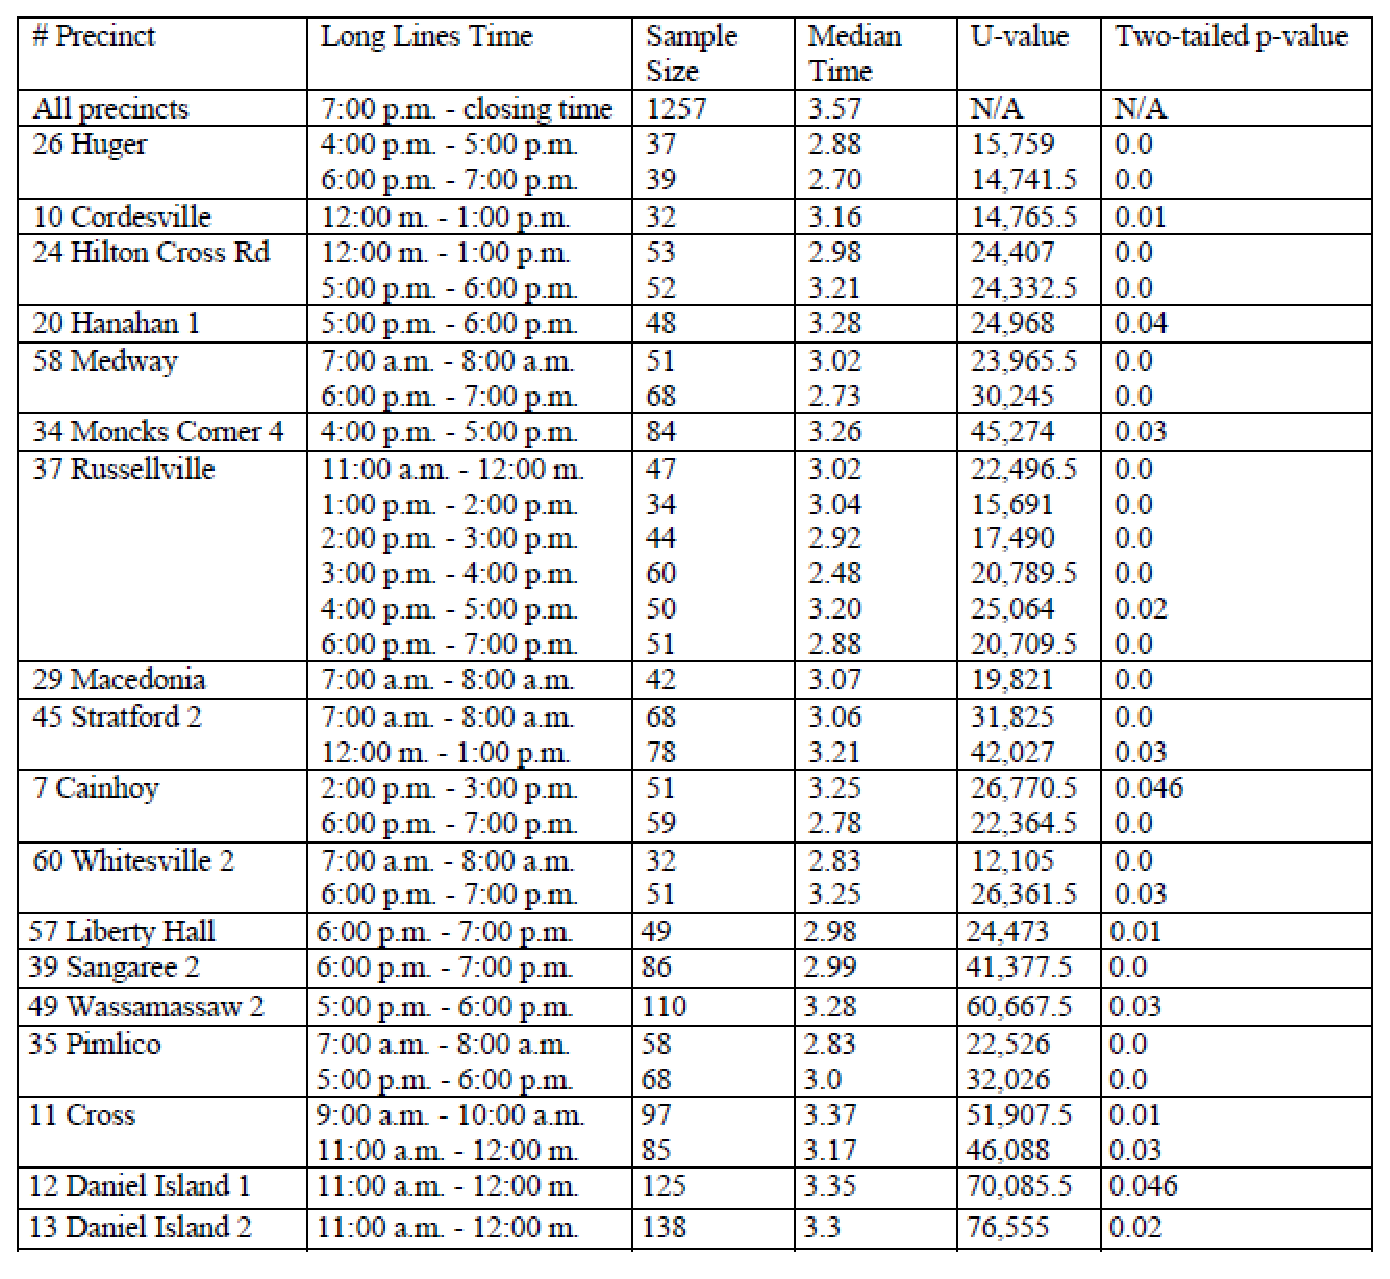
\includegraphics[width=0.5\textwidth,height=0.4\textheight]{berkeleyLongLineTable.eps}
\end{center}
\caption{Long lines in Berkeley County.}
\label{fig:mann-whitney-u}
\end{figure}

\section{Future Voting Systems Suggestions}
While many other DRE systems do capture data in their audit logs similar to what
the iVotronic does, no other widely deployed voting system makes it as easy to
gather all the audit logs from all of the voting machines into a single
place. As a result, while our methods are in principle applicable to other
deployed voting systems, in practice this would require additional effort from
election officials. Future voting system standards introduce stronger
requirements for audit logs; this could make it easier to apply our analyses to
other voting systems~\cite{Wagner2010}. 

We believe that the following recommendations will make audit files more usable. 
 
Vendors should document the meaning of all events. We found audit logs with
event messages, such as ``UNKNOWN,'' ``Warning – PEB I/O flag set,'' and
``Warning – I/O flagged PEB will be used,'' which sound ominous, however we
could not determine the gravity of the issue. Despite combing through all of
ES\&S’s publicly available information about the iVotronic, the meaning of these
events still remain a mystery~\cite{VerVot2011, ESS2011a, ESS2011b}. 
 
Accuracy of date and time logging needs improvement. When the machine has an
incorrect clock, timestamps are inaccurate and it becomes difficult to recreate
election day events. In addition, some audit log analyses, such as the open late
analysis, are made more difficult by unreliable timestamps. 
 
Make system manuals available to the public. Voting machine audit logs are
public information. The general public can request them under the Freedom of
Information Act. In the same fashion, we recommend that voting system manuals be
made freely available. This would allow the public to see for themselves if
there were any problems that should be addressed.  
 
Capture the ballot activation event. Recording the time each ballot is activated
(as opposed to only recording when the ballot is cast) would make it easier to
learn when the voting machines were heavily used and when they were idle.  
 
 \section{Related Work}
Two recent studies used event logs from the iVotronic voting system to audit
elections~\cite{Buel2011, Sandler2007}. Buell et al.~\cite{Buel2011} analyzed
the same South Carolina elections that we did and also discovered votes not
included in the certified counts and problems with the audit data. By consulting
additional audit materials, such as the printed results tapes, the authors were
able to offer possible explanations for why the problems occurred. Our work
takes a slightly different approach. We focus on developing an automated
analysis of the publicly available audit log data that can be used by
anyone. While our tool did discover and report similar problems, we simply
report what was wrong, but can not provide a possible explanation for the cause
of the error as we do not have access to printed results tapes.  

Sandler et al.~\cite{Sandler2007} analyzed vote tallies by comparing each
machine’s protected vote count to the printed results tapes. Their report also
finds time-stamps that were most likely inaccurate. With further investigation,
they concluded that the machine hardware clock was incorrect. Our research
provides analyses to identify similar problems, but in a way that can be
automated.   

There has also been research on using the audit logs to analyze election-day
procedure and activity. Antonyan et al. showed how event logs could be used to
determine if a machine acted ``normally'' on election
day~\cite{Antonyan2009}. They built a finite state machine that models the
sequences of events that a well-behaved AccuVote-OS scanner might produce and
used it to analyze AccuVote-OS logs. This type of analysis could be useful for
the iVotronic systems that we studied, too.  

Voter Verified Paper Audit Trails (VVPATs) are a different type of audit
log. Unlike the audit logs we used in our analyses, VVPATs are viewed and
verified by the voter and are more suited to audits concerning a DRE incorrectly
capturing a voter’s intent. Our work is more concerned with identifying cases of
cast votes not being included in the final count, or issues at the polling place
that might prevent the voter from casting their vote in the first place. With
VVPATs, as long as a certain percentage of voters do check their paper
ballot~\cite{Hall2006}, the voting machine need not be assumed correct, whereas
our analyses do make this assumption. 

\section{Conclusion}
This paper develops methods to analyze audit data from DRE voting machines. It 
introduces new methods for identifying anomalies in audit data; these include 
possible miscounts, procedural errors, voting machine malfunctions, and system 
deficiencies. In addition, we present a new analysis of voter flow, using only 
the generated audit logs.  Then we conduct an audit on the 2010 South Carolina 
election using these methods and use statistical analyses to provide meaningful
results. With this information, election officials can improve poll worker 
training, election official checklists, election tabulation procedures, and 
voting machine preparation testing.  
 
We built a web application, AuditTool, to perform these analyses. Users can
upload the DRE log files to our website and run the analyses. By automating our
analyses we can provide intelligent feedback to election officials during the
canvassing process and help them quickly correct any problems in order to
produce accurate election results. AuditTool is freely available online.  
 

%\section{Acknowledgments}
%Leave out for anonymization.

{\footnotesize \bibliographystyle{acm}
\bibliography{../Latex/paper2.bib}}


%\theendnotes

\end{document}







